\documentclass[12pt]{../notes}
\usepackage{docmute}
\title{Элементы линейной алгебры}
\date{22.06.2016}
\author{\texttt{taxus}}
\graphicspath{{img/}}
\begin{document}
\maketitle

\abstract{\sl
  Сей труд не стоит рассматривать как исчерпывающий конспект лекций. 
  Скорее он представляет субъективно выбранный мною материал, 
  показавшийся или наиболее важным, или наиболее непонятым, или ещё не знаю каким.
  Надеюсь, он хоть кому-нибудь принесёт немного пользы.
}

\tableofcontents
\newpage
\setcounter{chapter}{5}
\chapter{Линейные пространства}
\documentclass[12pt]{../../../notes}
\usepackage{silence}
\WarningFilter{latex}{Reference}
\graphicspath{{../../img/}}

\begin{document}

\setcounter{paragraph}{0}
\paragraph{Определения}
\begin{defn}\label{defn:linspace}
  Пусть $K$"--- поле. Рассмотрим множество  $V$ с двумя операциями
  \begin{align*}  
    + &: V \times V \to V \\
    \cdot &: K\times V \to V
  \end{align*}
  Тогда $V$"--- линейное пространство над $K$, если 
  $\forall\, \mathbf{x},\mathbf{y},\mathbf{z}\in V,\; \alpha_i \in K$
  \begin{enumerate}
    \item $(\mathbf{x}+\mathbf{y}) + \mathbf{z} = \mathbf{x} + (\mathbf{y}+\mathbf{z})$
    \item $\mathbf{x} + \mathbf{y} = \mathbf{y} + \mathbf{z} $
    \item $\exists\, \mathbf{0}\in V : \mathbf{x} + \mathbf{0} = \mathbf{x}$
    \item $\exists\, (-\mathbf{x})\in V : \mathbf{x} + (-\mathbf{x}) = \mathbf{0}$
    \item $(\alpha_1+\alpha_2) \mathbf{x} = \alpha_1 \mathbf{x} + \alpha_2 \mathbf{x}$
    \item $\alpha (\mathbf{x}_1 + \mathbf{x}_2) = \alpha \mathbf{x}_1 + \alpha \mathbf{x}_2$
    \item $1 \cdot \mathbf{x} = \mathbf{x}$
    \item $(\alpha_1 \alpha_2) \mathbf{x} = \alpha_1 (\alpha_2 \mathbf{x})$
  \end{enumerate}
\end{defn}

{ \defn\label{defn:linsubspace}
  Пусть $U,V$"--- линейные пространства над $K$, $U \subset V$. Тогда $U$"--- подпространство 
  $V$.
}

{ \defn\label{defn:lincomb}
Пусть $V$"--- линейное пространства над $K$, $\mathbf{x}_1, \dotsc, \mathbf{x}_n\in~V$, 
$\alpha_1, \dotsc, \alpha_n \in K$. Тогда $\alpha_1 \mathbf{x}_1 + \dotsb + \alpha_n \mathbf{x}_n$"--- 
линейная комбинация $\mathbf{x}_1, \dotsc, \mathbf{x}_n$.
}


\begin{lem}\label{lem:linspsign}
  Пусть $U,V$"--- линейные пространства над $K$, $U \subset V$. Тогда если $U$ замкнуто относительно
  $+, \cdot$  из  $V$, то  $U$"--- подпространство
  $V$.
\end{lem}
\begin{itlproof}
  Формулировка леммы аналогична тому, что всякая линейная комбинация элементов $U$ лежит в нём же.
  Нужная дистрибутивность, ассоциативность и т.д. унаследуется от соответствующих операций в 
  надпространстве, так как их свойства заданы на всём множестве $V$, а значит и на подмножестве $U$.
  Однако в некоторых свойствах требовалось существование в множестве чего-нибудь.
  Покажем, что все эти требования равносильны существованию линейной комбинации.
  \begin{enumerate}
      \setcounter{enumi}{2}
    \item $\exists\, \mathbf{0}\in U \Leftarrow \exists\, 0\cdot \mathbf{x},\; \mathbf{x}\in U$
    \item $\exists\, \mathbf{-x}\in U \Leftarrow \exists\, (-1)\cdot \mathbf{x},\; \mathbf{x}\in U$
  \end{enumerate}
\end{itlproof}

{ \defn\label{defn:linshell}
Пусть $V$"--- линейное пространства над $K$, $M \subset V$
\[
  \langle M \rangle = 
  \left\{ \alpha_1 \mathbf{x}_1 + \dotsb + \alpha_n \mathbf{x}_n \middle|
  \Big\{ \begin{array}{l}
    \alpha_1, \dotsc, \alpha_n \in K\\
    \mathbf{x}_1, \dotsc, \mathbf{x}_n \in M
  \end{array} \right\}
\] 
$\langle M \rangle$"--- линейная оболочка $M$.
}

\begin{lem}\label{lem:linspan}
  Верны утверждения:
  \begin{enumerate}
    \item $\langle M \rangle$"--- подпространство $V$
    \item $ \langle M \rangle = \bigcap\limits_i W_i$, $W_i \supset M$, $W_i$"--- подпространство $V$
  \end{enumerate}
\end{lem}
\begin{itlproof}
  Доказательства очень похожи на соответствующие в теории групп.
\end{itlproof}

%%% XXX так пробелы вокруг тире лучше: "---  чем так : ~---
%%%
\begin{defn}\label{defn:linspanprop}
  Пусть $V$"--- линейное пространство. Тогда
  $M \subset V$"--- порождающая система, если $\langle M\rangle = V$
\end{defn}


\paragraph{Линейная независимость системы векторов}

\begin{defn}\label{defn:linindp} Пусть $\mathbf{x}_1,\dotsc, \mathbf{x}_n \in V$, 
$\alpha_1, \dotsc, \alpha_n \in K$.
Тогда если 
\[
  \alpha_1\,\mathbf{x}_1 + \dotsb + \alpha_n\,\mathbf{x}_n = 0 \Rightarrow \forall\,i\;\alpha_i = 0
\]
то система векторов $\mathbf{x}_1, \dotsc, \mathbf{x}_n$ линейно независима.
В противном случае система линейно зависима.
\end{defn}

\subparagraph{Свойства}
\begin{enumerate}
  \item Подсистема линейно независимой системы линейно независима.
  \item В ЛНЗ системе ни один вектор не выражается через другие
\end{enumerate}

\paragraph{Лемма о линейной зависимости линейных комбинаций. Базис}
\begin{lem}[Линейная зависимость линейных комбинаций]\label{lem:ldlincomp} 
  Пусть $V = \{\mathbf{v}_1, \mathbf{v}_2,\dotsc, \mathbf{v}_n\}$~--- ЛНЗ, а 
  $U = \{\mathbf{u}_1, \dotsc , \mathbf{u}_m\}$"--- линейные комбинации векторов из $M$.
  Тогда если $m > n$, то $U$"--- линейно зависимы.  
\end{lem}

\begin{itlproof} 
  Там получается ОСЛУ, в которой уравнений больше, чем неизвестных.  Решение найдётся.
\end{itlproof}

\begin{defn}\label{defn:basis}
  Базис"--- линейно независимая (\ref{defn:linindp}), порождающая (\ref{defn:linspanprop})
  система векторов.
\end{defn}

\begin{defn}\label{defn:lindim}
  Размерность ($\dim$) линейного пространства"--- число векторов в базисе.
\end{defn}

\begin{lem}[Корректность определения размерности]\label{lem:lindimcorr}
  Пусть $\{u_i\}_{1 \leqslant i \leqslant n}, \{v_i\}_{1 \leqslant i \leqslant m}$"--- базисы
  $V$. Тогда $m=n$.
\end{lem}
\begin{itlproof}
  Иначе одна система выражается через другую и по~\ref{lem:ldlincomp} она ЛЗ, что странно.
\end{itlproof}


\paragraph{Базис в конечномерных пространствах}
Во всех следующих теоремах действие происходит в конечномерных пространствах.

\begin{thrm}\label{thrm:basisfromspan}
  Из всякой порождающей системы можно выделить базис
\end{thrm}

\begin{imp}
  Базис"--- минимальная порождающая система векторов
\end{imp}

\begin{thrm}\label{thrm:basicfrimlinind}
  Из всякой линейно независимой системы можно выделить базис.
\end{thrm}
\begin{imp}
  Базис"--- максимальная линейно независимая система
\end{imp}

\paragraph{Сумма и пересечение ЛП}
\begin{defn}\label{defn:linspsum}
  Пусть $\forall\, i \in I \;\: U_i \subset V$. Тогда 
  \[
    \sum_{i\in I} U_i := \left\{ u_{1} + \dotsb + u_{n} \mid u_{i} \in U_i\right\}
  \]
  То есть совокупность всевозможных сумм
\end{defn}
\begin{defn}\label{defn:linspintersec}
  \[
    \bigcap_{i\in I} U_i := \{u \mid \forall\, i \;\: u \in U_i\}
  \]
\end{defn}

\begin{rem*}
  Пересечение"--- подпространство.
\end{rem*}

\begin{thrm}\label{thrm:dimsumlinsp}
  Пусть $U_1, U_2 $"--- подпространства $V$.
  Тогда
  \[
    \dim (U_1+U_2) = \dim U_1 + \dim U_2 + \dim (U_1 \cap U_2)
  \]
\end{thrm}
\begin{ittproof}
  Пусть $\dim(U_1 \cap U_2) = k$, $\dim U_1 = k + l$, $\dim U_2 = k + n$. Тут мы просто дополняем
  базис пересечения до базиса пространства, умеем же по \ref{thrm:basicfrimlinind}.
  \begin{enumerate}
    \item Сначала доказываем, что $k + l + n$ нужных векторов вообще хватит, чтобы породить всё
      $U_1 + U_2$
    \item Потом доказываем, что построенный таким образом базис линейно независим
  \end{enumerate}
\end{ittproof}

\paragraph{Внутренняя прямая сумма}
\begin{defn}\label{defn:dirsum}
  Пусть $\{U_i\}_{i\in I} \subset 2^V$, $U = \sum_I U_i$. Тогда
  \[
    \left( \sum_{\substack{i\in I \\ u_i\in U_i}} u_i = 0 
    \Rightarrow \forall\, i \;\: u_i = 0\right)
    \Leftrightarrow U = \bigoplus_{i\in I} U_i
  \]
\end{defn}

\begin{lem}\label{lem:dirsumuniq}
  Элемент из прямой суммы единственным образом представляется суммой $u_i \in I_i$.
\end{lem}

\begin{thrm}[Критерий $\oplus$]\label{thrm:dirsumcrit}
  Пусть  
  \begin{align*}
    U   &= \sum_{i \in I}  U_i \\
    W_i &= \sum_{j\in I, j\neq i} U_j
  \end{align*}
  Тогда $U$"--- прямая сумма $\Leftrightarrow$ 
  \[
    \forall\, i \;\: U_i \cap W_i = \{0\}
  \]
\end{thrm}
\begin{ittproof}
  Более-менее ясно из определения прямой суммы. И вообще, похоже на свойства ЛНЗ системы
  векторов. 
\end{ittproof}

\paragraph{Размерность прямой суммы конечного числа ЛП}
\begin{thrm}\label{thrm:dimdirsum}
  \[
    \dim \underbrace{\bigoplus_{i\in I} U_i}_{V} = \sum_{i\in I} \dim U_i
  \]
\end{thrm}
\begin{ittproof}
%%Тут у Карпова индукция была, проще же можно..
(По мотивам \cite[стр.~195]{vinberg}).

  Сначала заметим, что объединение базисов~--- точно порождающая система в $V$.
  Теперь докажем, что она линейно независима.
  Пусть для начала ${e_{ij}}$~--- базис $U_i$.
  Тогда 
  \[
    V \ni v = \sum_{i,j} \alpha_{ij} e_{ij} 
  \]
  Сгруппируем
  \begin{align*}
    u_i &= \sum_j \alpha_{ij} e_{ij} \\
      v &= 0 \Leftrightarrow \sum_i u_i = 0 \Leftrightarrow \forall\, i \;\: u_i = 0
  \end{align*}
  Ну а ноль в подпространствах представляется единственным образом
  \[
    u_i = 0 \Rightarrow \forall\, j \;\: \alpha_{ij} = 0
  \]
\end{ittproof} 

\begin{stat}[Непонятно зачем нужное утверждение]\label{stat:dirsumsubfact}
  Пусть 
  \[
    V_{k+1} = \bigoplus_{i=1}^{k+1} U_i, \; V_k = \sum_{i=1}^k U_i
  \]
  Тогда
  \[
    V_k = \bigoplus_{i=1}^k U_i
  \]
\end{stat}

\paragraph{Аффинные подпространства}

\begin{defn}\label{defn:affinsubspc}
  Пусть $U$"--- подпространство $V$, $a\in V$. Тогда $W = U + a = \{x+a\mid x\in U\}$~--- аффинное 
  подпространство. 
\end{defn}

\begin{lem}\label{lem:affinfact}
  Пусть $U$"--- подпространство $V$. Тогда
  \[
    U + a = U + b \Leftrightarrow a - b \in U
  \]
\end{lem}
\begin{lem}\label{lem:affinprop}
  Пусть $V$~--- линейное пространство над $K$, $W \subset V$, $a\in V$.
  Тогда если:
  \begin{enumerate}
    \item $\forall\, \alpha \in K, x \in W \;\: \alpha(x-a) + a \in W$  
    \item $\forall\, x_1,x_2 \in W \;\: x_1 + x_2 - a \in W$  
  \end{enumerate}
  то $W$~--- аффинное подпространство
\end{lem}

\paragraph{Факторпространство}
\begin{defn}\label{defn:factorspace}
  Пусть $U$~--- подпространство линейного пространства $V$ над полем $K$.
  Тогда такая структура называется факторпространством:
  \begin{align*}
    V / U &:= \{ U + a \mid a\in  V \} \\
    \overline a &:= U+a \\
    \overline a + \overline b &:= \overline{a+b} \\
    \alpha \cdot \overline a &:= \overline{\alpha \cdot a}
  \end{align*}
\end{defn}

\begin{stat}\label{stat:corrfactspc}
  Определение~\ref{defn:factorspace} корректно
\end{stat}

\begin{stat}\label{stat:factspcISspace}
  Структура которую описали в~\ref{defn:factorspace}"--- векторное пространство.
\end{stat}

\begin{thrm}\label{thrm:dimfactspc}
  \[
    \dim (V/U) = \dim V - \dim U
  \]
\end{thrm}

\begin{defn}\label{defn:relbasis}
  Дополнение базиса $U$ до базиса $V$ называется базисом $V$ относительно $U$ (относительным
  базисом).
\end{defn}


\end{document}


\chapter{Матрицы}
\documentclass[12pt]{../../../notes}
\usepackage{silence}
\WarningFilter{latex}{Reference}
\graphicspath{{../../img/}}

\begin{document}

\paragraph{Матрицы, основные определения}
\begin{defn}[Матрицы над $K$]\label{defn:matrices}
  Пусть $K$"--- поле, $m,n\in \N$. Тогда
  \[
    M_{m,n}(K) = 
    \left\{
      A 
    \,\middle|\,
      A  = 
      \begin{pmatrix}
        a_{11} & a_{12} & \cdots & a_{1n} \\
        a_{11} & a_{12} & \cdots & a_{1n} \\
        \vdots & \vdots & \ddots & \vdots \\
        a_{m1} & a_{m2} & \cdots & a_{mb}
      \end{pmatrix},\;
      a_{ij} \in K
    \right\}
  \]
\end{defn}

\begin{defn}[Сложение матриц]\label{defn:matradd}
  $A_{mn}\cdot B_{mn}:$
  \[
    (a+b)_{ij} = a_{ij} + b_{ij}
  \]
\end{defn}

\begin{defn}[Умножение матриц]\label{defn:matrmul}
  $A_{mn}\cdot B_{nk}:$
  \[
    (ab)_{ij} = \sum_{l=1}^n a_{i\ell}\cdot b_{\ell j}
  \]
\end{defn}

\paragraph{Кольцо квадратных матриц}
Обозначается $M_n(K)$

\noindent Ноль:
\[
  Z_n = 
  \begin{pmatrix}
    0      & 0      & \cdots & 0 \\
    0      & 0      & \cdots & 0 \\
    \vdots & \vdots & \ddots & \vdots \\
    0      & 0      & \cdots & 0 \\
  \end{pmatrix}
\]
Единица:
\[
  E_n = 
  \begin{pmatrix}
    1      & 0      & \cdots & 0 \\
    0      & 1      & \cdots & 0 \\
    \vdots & \vdots & \ddots & \vdots \\
    0      & 0      & \cdots & 1 \\
  \end{pmatrix}
\]
\parrange{2}{Определитель}
\begin{defn}\label{defn:determinant}
  Пусть $A\in M_n(K)$
  \[
    \det A = \sum_{\sigma \in S_n} (-1)^{I(\sigma)} \cdot a_{1\sigma(1)} \dotsm a_{n\sigma(n)}
  \]
\end{defn}
\begin{defn}\label{defn:determrows}
  Если обозначать строки $A_1, \dotsc , A_n$, а столбцы $A^{(1)}, \dotsc , A^{(n)}$,
  то можно ввести ещё такую функцию:
  \[
    \det (A_1, \dotsc , A_n) = \det (A^{(1)}, \dotsc , A^{(n)}) := \det A
  \]
\end{defn}

\begin{defn}[Элементарные преобразования]\label{defn:elemtranf}
  \noindent\newline\par
  \begin{enumerate}[I]
    \item\label{it:transfchng}   \makebox[8em][l]{$A_i \leftrightarrows A_j$} 
      $A^{(i)} \leftrightarrows A^{(j)}$     
    \item\label{it:transfaddmul} \makebox[8em][l]{$A_i := A_i + \lambda A_j$} 
      $A^{(i)} := A^{(i)} + \lambda A^{(j)}$ 
    \item\label{it:transfmul}    \makebox[8em][l]{$A_i := \lambda A_i$}       
      $A^{(i)} := \lambda A^{(i)}$           
  \end{enumerate}
\end{defn}
\begin{defn}[Транспонированная матрица]\label{defn:transpose}
  \[
    A^T \colon (a^T)_{ij} = (a)_{ij}
  \]
\end{defn}

\subparagraph{Свойства}
\begin{enumerate}
  \item Определитель (в описанном в~\ref{defn:determrows} смысле) полилинеен и кососимметричен по
    строкам и столбцам.
  \item Если 2 строчки или столбца одинаковые, то определитель равен 0
  \item Элементарные преобразования влияют на определитель следующим образом:\par
    \begin{tabular}{c|r}
      I   & $(-1)\det A$ \\
      II  & $\det A$     \\
      III & $\lambda \det A$
    \end{tabular}
  \item $\det A^T = \det A$
\end{enumerate}


\paragraph{Теорема Лапласа}
\begin{defn}[Минор]\label{defn:minor}
  Пусть $A\in M_n(K)$, а $k\in \N$. Тогда определитель подматрицы, собранной из $k$ строк и $k$
  столбцов называется \emph{минором} порядка $k$.
  \[
    \Delta = 
    \begin{vmatrix}
      a_{i_1j_1} & \cdots & a_{i_1j_k} \\
      \vdots & \ddots & \vdots \\
      a_{i_kj_1} & \cdots & a_{i_kj_k} 
    \end{vmatrix}
  \]
  $\Delta'$~--- дополнительный минор"--- всё, что осталось.
  Его ещё иногда (когда минор"--- один элемент) обозначают как $M_{ij}$
\end{defn}
\begin{defn}[Алгебраическое дополнение]\label{defn:cofactor}
  \[
    A_\Delta = (-1)^{i_1 + \dotsb + i_k + j_1 + \dotsb + j_k} \Delta'
  \]
\end{defn}

\begin{thrm}[Теорема Лапласа]\label{thrm:laplacecofactor}
  Пусть $A\in M_n(K)$, $k\in \N$. Выберем из матрицы $k$ строчек. Тогда
  \[
    \det A = \sum_{\Delta} \Delta \cdot A_\Delta
  \]
  где $\Delta$~--- любой минор, содержащий нужные $k$ строчек.
\end{thrm}
\begin{ittproof}
  Выберем какой-то один минор, $i_k$~--- его строчки, $j_\ell$~--- его столбцы
  \[
    \Delta : 
    \begin{cases}
      i_1, \dotsc , i_k \\
      j_1, \dotsc , j_k
    \end{cases}
  \]
  Теперь отправим все элементы, попавшие в минор, в левый верхний угол.
  Сначала сдвинем все строчки:
  \[
    \begin{cases}
      i_1 \to 1 & (i_1 -1 \text{~сдвигов})\\
      \hdotsfor{2} \\
      i_k \to k & (i_k - k \text{~сдвигов})
    \end{cases}
  \]
  Потом все столбцы
  \[
    \begin{cases}
      j_1 \to 1 & (i_1 - 1 \text{~сдвигов})\\
      \hdotsfor{2} \\
      j_k \to k & (i_k - k \text{~сдвигов})
    \end{cases}
  \]
  В итоге, из свойств элементарных преобразований, получим: 
  \[
    \det B = (-1)^{i_1 - 1 + \dotsb + i_k - k + j_1 - 1 + \dotsb + j_k - k} \det A 
    = (-1)^{i_1  + \dotsb + i_k  + j_1  + \dotsb + j_k } \det A 
  \]
  так как все добавки парные $\Rightarrow$ делится на $2$.

  С другой стороны, $\Delta$ и $\Delta'$ никак не поменялись, так как переставляемые чиселки в
  них не не входят. Также нужно отметить, что $B_\Delta = \Delta'$, по тем же причинам, в
  общем-то.

  Посмотрим, что такое  $\Delta\cdot \Delta'$
  \footnote{Вообще, тут маленькая неточность: здесь фактически 
      \emph{действие} группы перестановок на множестве $\{k+1, \dotsc , n\}$}.
  \begin{align*}
    \Delta \cdot \Delta' 
    &= \Bigg( \sum_{\tau \in S_k} (-1)^{I(\tau)} b_{1\tau(1)} \dotsm
    b_{k\tau(k)} \Bigg) \cdot \Bigg( \sum_{\tau' \in S_{n-k}} (-1)^{I(\tau')} b_{k+1\tau'(k+1)} \dotsm
    b_{n\tau(n)} \Bigg)
  \end{align*}
  Пусть теперь $\sigma = \tau \circ \tau'$. Тогда $I(\sigma) = I(\tau)+I(\tau')$ по свойствам
  перестановок, а $\sigma$ фактически разбивается на 2 независимых: $\tau$ и $\tau'$.
  В итоге
  \[
    \Delta \cdot \Delta' 
    = \sum_{\sigma\in S_n} (-1)^{I(\sigma)} b_{1\sigma(1)} \dotsm b_{n\sigma(n)}
  \]
  А это вообще-то правильный кусок определителя $B$. 
  Поймём, что это за кусок определителя $A$.
  Числа-то те же самые. А вот на вопрос со знаком мы уже по сути ответили, когда рассуждали про 
  определитель. Слагаемые точно не перемешиваются, так как все перестановки"--- биекции, 
  так что каждое слагаемое просто умножается на $(-1){\cdots}$. 
  Так что 
  \begin{align*}
    \Delta \cdot \Delta' &= (-1)^{i_1  + \dotsb + i_k  + j_1  + \dotsb + j_k } 
    \sum_{\sigma'} a_{1\sigma'(1)} \dotsm a_{n\sigma'(n)} \\
    A_{\Delta} &= (-1)^{i_1  + \dotsb + i_k  + j_1  + \dotsb + j_k } \Delta'  \\
    \Delta \cdot A_{\Delta} &= \sum_{\sigma'} a_{1\sigma'(1)} \dotsm a_{n\sigma'(n)}
  \end{align*}
  где у $\sigma'$ уже другие независимые циклы: ${i_1, \dotsc , i_k\choose j_1, \dotsc , j_k }$ 
  и всё остальное.

\end{ittproof}
\begin{imp}
  \[
    \det A = a_{i1} A_{i1} + \dotsb + a_{in} A_{in} 
  \]
\end{imp}
\begin{imp}
  \[
    a_{j1} A_{i1} + \dotsb + a_{jn} A_{in} = 0
  \]
\end{imp}
\begin{itlproof}
  Приравняем $i$ строчку к $j$-ой, получим матрицу $B$. Тогда
  \[
    a_{j1} A_{i1} + \dotsb + a_{jn} A_{in} = b_{i1} B_{i1} + \dotsb + b_{jn} B_{in} = \det B = 0
  \]
  Так как определитель $B$ очевидно равен 0
\end{itlproof}

\paragraph{Ступенчатая матрица}

\begin{defn}\label{defn:stairsmtx}
  $A$ = \raisebox{-0.45\height}{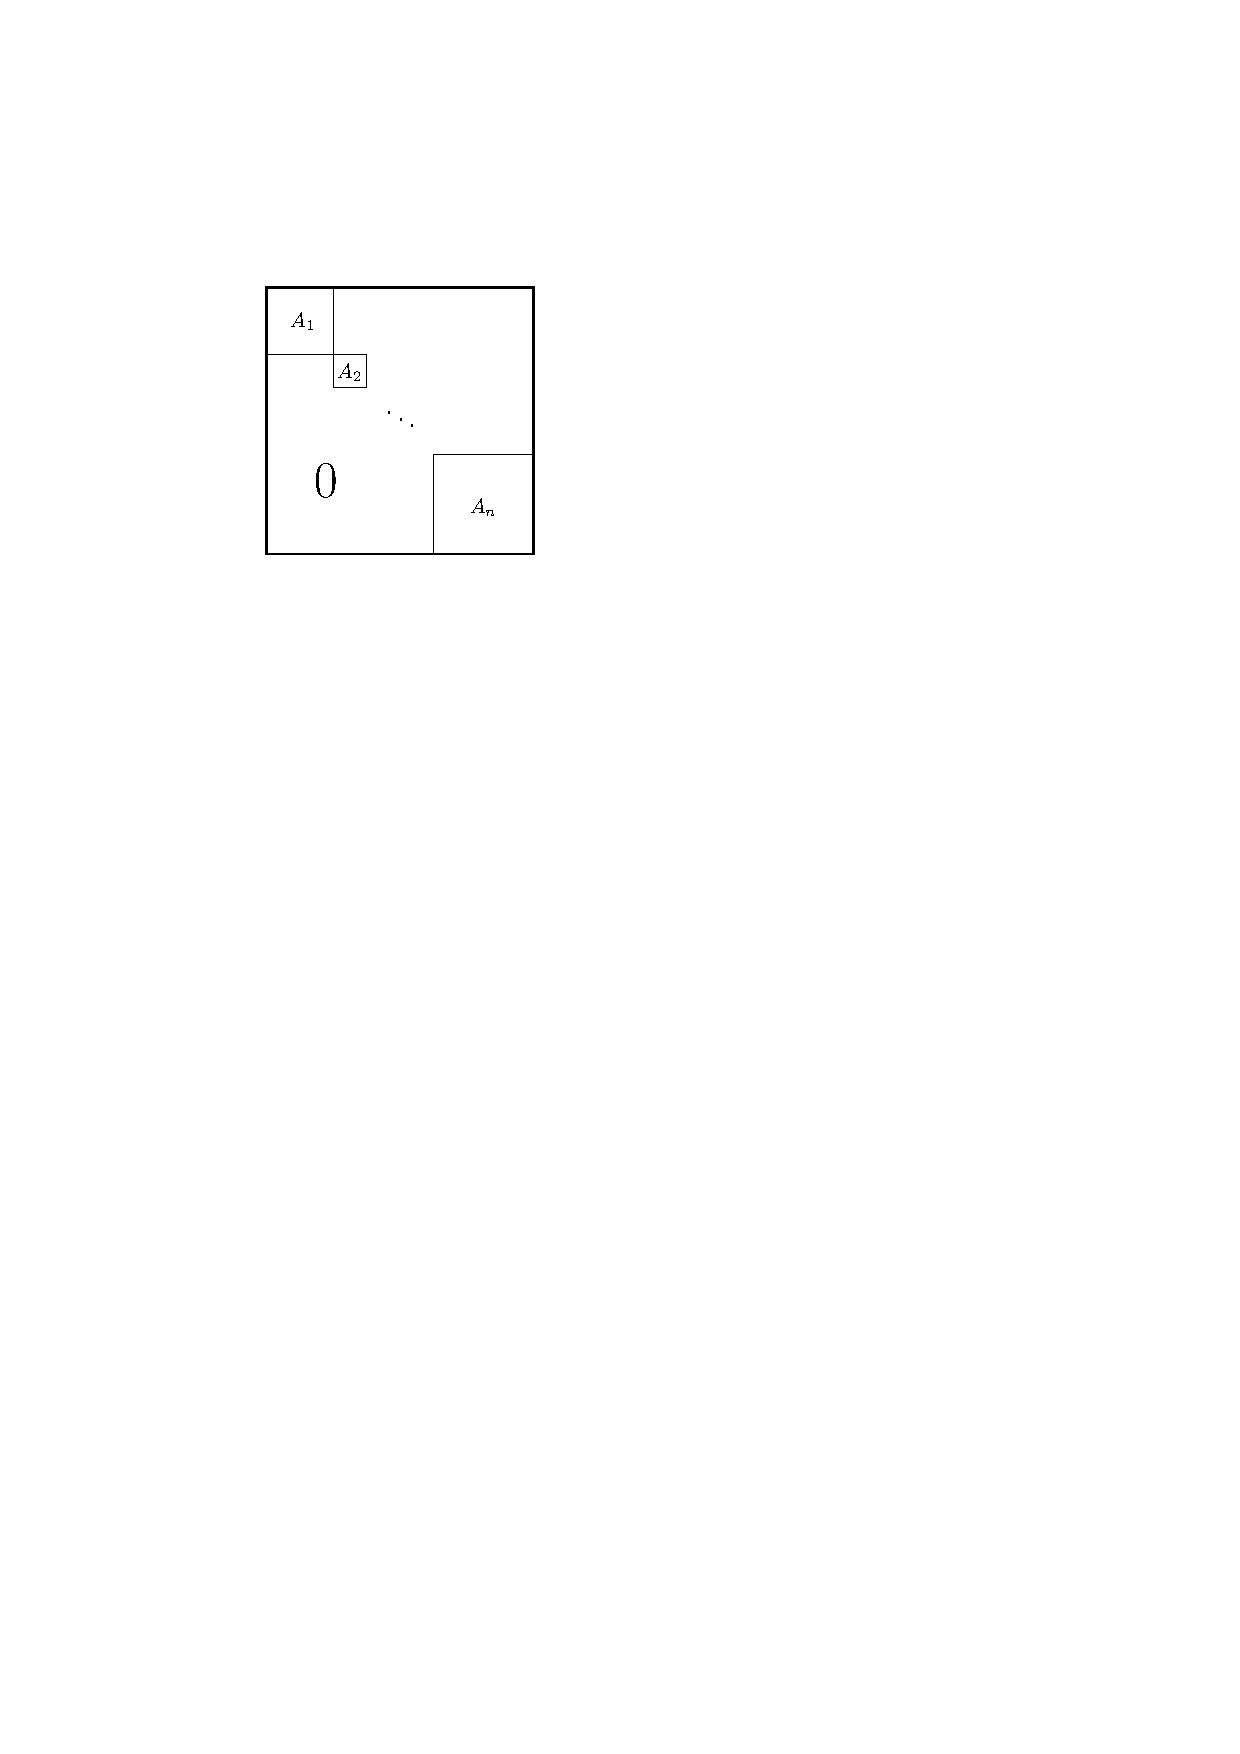
\includegraphics[scale=0.6]{stairsmtx}}~--- ступенчатая 
  матрица.\footnote{вообще-то, она квазитреугольная, а не ступенчатая}
\end{defn}
\begin{thrm}[Определитель ступенчатой матрицы]\label{thrm:stairsdet}
  \[
    \det A = \det A_1 \dotsm \det A_n
  \]
\end{thrm}
\begin{ittproof}
  По индукции через теорему Лапласа~\ref{thrm:laplacecofactor}
\end{ittproof}

\paragraph{Определитель произведения матриц}
\begin{thrm}\label{thrm:detmult}
  Пусть $A,B \in M_n(K)$. Тогда
  \[
    \det (AB)  = \det A \cdot \det B
  \]
\end{thrm}
\begin{ittproof}
  Докажем, что такие матрицы имеют одинаковый определитель:
  \[
    C = 
    \left(
    \begin{array}[h]{c|c}
      A    & 0 \\
      \hline 
      -E_n & B
    \end{array}
    \right) \quad \text{и} \quad 
    D = 
    \left(
    \begin{array}[h]{c|c}
      AB    & A \\
      \hline 
      0 & -E_n
    \end{array}
    \right)
  \]
  Теперь сделаем из куска с $B$ $Z_n$. 
  \[
    D'^{(n+j)} := C^{(n+j)} + b_{1j} C^{(1)} + \dotsb + b_{nj} C^{(n)}
  \]
  Внизу получатся нули, а вот сверху:
  \[
    d_{i,n+j} = 0 + b_{1j} a_{i1} + \dotsb + b_{nj} a_{in} = (ab)_{ij}
  \]
  Тысяча индексов, это же произведение матриц!
  \[
    D' = \left(
    \begin{array}[h]{c|c}
      A    & AB \\
      \hline 
      -E_n & 0
    \end{array}
    \right) 
  \]
  Мы тут пользовались только преобразованием \ref{it:transfaddmul}, так что определитель не
  поменялся. 

  Теперь переставим половинки матрицы. При этом будет совершено $n$ 
  преобразований~\ref{it:transfchng}. Так что
  \[
    \begin{split}
      \det A \det B & = \det C = \det D' = (-1)^n \det D = (-1)^n \det(-E_n) \det(AB) \\
                    & =  (-1)^{2n} \det(AB) = \det AB
    \end{split}
  \]
\end{ittproof}

\paragraph{Обратимость матриц}

\begin{defn}\label{defn:nonzerodet}
  Пусть $A = M_n(K)$. Тогда $A$~--- невырожденная $\Leftrightarrow$ $\det A \neq 0$
\end{defn}
\begin{defn}[Взаимная матрица]\label{defn:adjointmtx}
  \[
    \widetilde{A} = (a)_{ij}^T
  \]
\end{defn}

\begin{lem}\label{lem:adjointmtx}
  \[
    A\cdot\widetilde A = \det A \cdot E_n
  \]
\end{lem}

\begin{defn}\label{defn:invertmtx}
  Пусть $A = M_n(K)$. Тогда матрица $A^{-1}:$
  \[
    A\cdot A^{-1} = A^{-1} \cdot A = E_n
  \]
  (если существует)
\end{defn}

\begin{imp}
  Если $\det A \neq 0$, то
  \[
    A^{-1} = \frac{1}{\det A} \widetilde{A}
  \]
\end{imp}

\begin{imp}
  А невырождена $\Leftrightarrow$ А"--- обратима. 
\end{imp}

\begin{imp}
  Пусть $A,B \in M_n(K)$. Тогда 
  \[
    AB = E_n \Rightarrow A,B \text{~--- обратимы и } 
    \begin{cases}
      B = A^{-1} \\
      A = B^{-1}
    \end{cases}
  \]
\end{imp}

\parrange{2}{Ранг, строчный и столбцовый}
\begin{defn}[Строчный ранг]\label{defn:rowrank}
  Пусть $A\in M_{m,n}(K)$. Тогда \[
    \rk_s (A) = \dim \langle A_1, \dotsc , A_m \rangle
  \]
\end{defn}

\begin{defn}[Столбцовый ранг]\label{defn:colrank}
  Пусть $A\in M_{m,n}(K)$. Тогда \[
    \rk^{(s)} (A) = \dim \langle A^{(1)}, \dotsc , A^{(m)} \rangle
  \]
\end{defn}

\begin{lem}\label{lem:rowranktransf}
  Строчный ранг сохраняется при элементарных преобразованиях строк.
\end{lem}
\begin{itlproof}
  Пусть $B_1, \dotsc , B_m$ получены из $A_1, \dotsc , A_m$ элементарными преобразованиями строк.
  Эти преобразования"--- линейные.\footnote{Вообще, конечно, так нехорошо. Линейные отображения 
  ещё не ввели, так что надо каждое преобразование проверять}.
  Так что линейная оболочка никак не изменится. 
  \[
    \langle A_1, \dotsc , A_m\rangle = \langle B_1, \dotsc , B_m\rangle
  \]
  А значит, и ранги совпадают.
\end{itlproof}
Транспонирование даст аналогичное рассуждение для столбцов

\begin{lem}\label{lem:colranktransf}
  Столбцовый ранг сохраняется при элементарных преобразованиях строк.
\end{lem}
\begin{itlproof}
  Пусть $\rk^{(s)} (A) = r$.
  Будем по одному убирать из линейной оболочки столбцов линейно выражающиеся векторы
  \[
    \langle A^{(1)}, \dotsc , A^{(n)}\rangle \rightsquigarrow 
    \langle A^{(i_1)}, \dotsc , A^{(i_r)}\rangle
  \]
  Пусть после линейных преобразований образы этих векторов стали линейно зависимы, 
  $A \rightsquigarrow B$. Перепишем:
  \begin{align*}
    \beta_1 B^{(i_1)}+ \dotsb + \beta_n B^{(i_r)} = 0 
    \Leftrightarrow
    \begin{cases}
      b_{1i_1} \beta_1 + \dotsb + b_{1i_r} \beta_n = 0\\
      \hdotsfor{1} \\
      b_{mi_1} \beta_1 + \dotsb + b_{mi_r} \beta_n = 0
    \end{cases} \quad (\exists\, \beta_i \neq 0)
  \end{align*}
  Проведём все преобразования в обратную сторону. Тогда, $\{\beta_i\}$ тоже останутся решениями
  такой системы уравнений, так как все преобразования не изменят решений.
  А тогда и $\{A^{i_k}\}$~--- линейно зависимы(?!?).

  Таким образом, $\rk^{(s)} B \geqslant \rk^{(s)} A$. Теперь можно поменять всюду $A$ и $B$ местами.
  В силу обратимости элементарных преобразований рассуждение не изменится. 
  Так что $\rk^{(s)} A \geqslant \rk^{(s)} B$. А тогда $\rk^{(s)} A = \rk^{(s)} B$.
\end{itlproof}
Транспонирование даст аналогичное рассуждение для строчек

\paragraph{Ранг матрицы}


\begin{thrm}\label{thrm:rowrk=colrk}
  Строчный и столбцовый ранг совпадают
\end{thrm}
\begin{ittproof}
  Тут рисовать надо, а я пока не умею это делать быстро..$\ddot{\frown}$
  Будем приводить матрицу к такому виду:
  \[
    \left(
    \begin{array}{c|c}
      E_r & 0 \\ \hline
      0   & 0
    \end{array}
    \right)
  \]
  \begin{enumerate}
    \item Найдём ненулевой элемент, поставим в $1,1$ преобразованием~\ref{it:transfchng}
    \item С помощью преобразования~\ref{it:transfaddmul} для строк сделаем нулевым весь первый
      столбец, кроме $1,1$. 
    \item Теперь с помощью такого же преобразования для столбцов сделаем первую строку нулевой,
      кроме первого элемента.
    \item Поделим первую строку на первый элемент
    \item Выкинем первую строку и первый столбец, повторив всё для остальной матрицы
  \end{enumerate}
  Даже такие издевательства над бедной матрицей не изменят оба ранга.
  А в преобразованной они очевидно равны
\end{ittproof}

\begin{defn}[Ранг матрицы]\label{defn:mtxrank}
  \[
    \rk A := \rk_s (A) = \rk^{(s)} A
  \]
\end{defn}

\paragraph{Ранги и миноры}
\begin{thrm}\label{thrm:rkminor}
  Ранг матрицы"--- наибольший порядок\footnote{размер подматрицы соответствующей минору, проще
  говоря.} её ненулевого минора.
\end{thrm}
\begin{ittproof}
  Пусть $\rk A = r$. Тогда строки всех миноров порядка $s > r$ линейно зависимы. А значит, можно 
  элементарными преобразованиями получить строку нулей. Значит, наибольший порядок минора
  $\leqslant r$. 

  Докажем, что минор порядка $r$ подходит. Выберем $r$ линейно независимых строк и из них вытащим
  подматрицу. Убедимся, что её определитель ненулевой.
  Можно преобразовать её всё тем же алгоритмом, что был описан в теореме~\ref{thrm:rkminor},
  разве что делить первую строку чтобы получить 1 не будем.
  Если где-то появится нулевая строка, значит строки были линейно зависимы. А матрица ещё была
  квадратной. Так что получится матрица диагонального вида. Определитель посчитать нетрудно, он
  получается ненулевой.
\end{ittproof}

\paragraph{Матричная запись СЛУ и решения такой системы}
\begin{defn}\label{defn:matrslineq}
Рассмотрим какую-то систему линейных уравнений

\begin{equation}
  \begin{cases}
    a_{11} x_1 + \dotsb +a_{1n} x_n = b_1\\
    \hdotsfor{1} \\
    a_{m1} x_1 + \dotsb +a_{mn} x_n = b_1
  \end{cases}
  \label{eq:sleq}
\end{equation}

Можно записать её в таком виде:
\[
  A\cdot X = B
\]
где $A$~--- матрица системы, $X$~--- столбец неизвестных, $B$~--- столбец решений, умножение
матричное.

Однородную систему уравнений можно записать как $A\cdot X = 0$
\begin{equation}
  \begin{cases}
    a_{11} x_1 + \dotsb +a_{1n} x_n = 0\\
    \hdotsfor{1} \\
    a_{m1} x_1 + \dotsb +a_{mn} x_n = 0
  \end{cases}
  \label{eq:hsleq}
\end{equation}

\end{defn}

\begin{thrm}\label{thrm:homsystsolspc}
  Решение однородной системы линейных уравнений"--- подпространство $K^n$, причём размерность
  пространства решений"--- количество главных (основных, базисных) переменных.
\end{thrm}
\begin{ittproof}
  Приведём матрицу к ступенчатому\cite[стр.~50]{Vinberg} виду. Нигде это нормально не 
  определялось, но и так очевидно что это и как получается. Я рисуночек хотел вставить, но не
  успею.
  
  Тогда главные переменные"--- те, что которые соответствуют числа, \emph{не} стоящие на краях 
  <<ступенек>>. Пусть $i_1, \dotsc , i_k$~--- их номера. Тогда рассмотрим $\{e_j\}$, такие, что
  \[
    e_j = 
    \begin{pmatrix}
      \vdots \\
      0 \\
      \vdots \\
      1 \\
      \vdots \\
      0\\
      \vdots
    \end{pmatrix}
    \begin{matrix}
      \vdots \\
      i_1 \\
      \vdots \\
      i_j \\
      \vdots \\
      i_k\\
      \vdots
    \end{matrix}
  \]
  причём остальные чиселки в этих векторах выбираются с тем условием, что $A e_j = 0$.

  Все $e_j$ разные, так что система линейно независима. Теперь докажем, что все решения
  порождаются такой системой векторов. 

  Пусть $x$~--- столбец решений. Соберём
  \[
    x^* = x_{i_1} e_i + \dotsb +x_{i_k} e_k 
  \]
  Если подумать до конца своих дней, то можно осознать, что
  \[
    \begin{cases}
      A x = 0 \\
      A x^* = 0
    \end{cases} \Rightarrow x-x*\text{~--- решение}.
  \]
  Оказалось, что думать до конца своих дней не нужно, ведь векторы $e_j$ определены так, что  
  $Ax^* = 0$. 
  
  Итак, мы выяснили, что $x-x^*$ решение. Но у этого вектора на всех позициях, соответствующих
  главным переменным стоят нули. А раз он решение, то и на всех остальных местах нули.
  (ну, иначе $1\cdot x_1 \neq 0$, например). Тогда $x = x^*$.

  Чудно, мы получили что можем таким хитрым базисом породить все решения. Докажем, что
  решения"--- подпространство.
  
  Пусть $x^1, x^2$~--- решения. Тогда
  \[
    A(\lambda x^{(1)} + \mu x^{(2)}) = \lambda A x^{(1)} + \mu A x^{(2)} = \lambda 0 + \mu 0 = 0
  \]
  Тогда по лемме~\ref{lem:linspsign} оно подпространство. А выбранные векторы $e_j$~--- базис,
  так как они порождают все решения и линейно независимы.
\end{ittproof}  

\begin{defn}\label{defn:fundsol}
  Базис пространства решений ОСЛУ~--- фундаментальная система решений.
\end{defn}

\begin{thrm}\label{thrm:dimsolnslq}
  Пусть~\eqref{eq:hsleq}~--- однородная система линейных уравнений. Тогда размерность
  пространства её решений равна $m - \rk A$, где $m$~--- порядок матрицы.
\end{thrm}
\begin{ittproof}
  Если сделать матрицу ступенчатой с единицами на <<ступеньках>> , то её ранг не изменится. 
  Размерность строк приведённой матрицы~--- это число <<ступенек>>. 
  А последнее равно $m-k$, где $k$~--- число главных переменных.
\end{ittproof}

\begin{thrm}\label{thrm:homtoordlinsys}
  Пусть $V$~--- пространство решений \eqref{eq:hsleq}, $U$~--- множество решений \eqref{eq:sleq},
  $x^0\colon Ax^0 = B$. Тогда $U =  V+ x^0$~--- аффинное подпространство $K^n$ 
\end{thrm}
\begin{ittproof}
  Пусть $x \in V + x^0$. Тогда $x = x'+ x^0$, $x' \in V$.
  \[
    A x = Ax' + Ax^0 = B + 0 = B \Rightarrow x\in U \Rightarrow V + x^0 \subset U
  \]
  С другой стороны, пусть $y \in U$. Тогда 
  \[
    A(y - x^0) = Ay - Ax^0 = 0 \Rightarrow y \in V+x^0 \Rightarrow U \subset V+ x^0 
  \]
\end{ittproof}

\paragraph{Теорема Кронекера-Капелли}

\begin{defn}\label{defn:compsysleq}
  Система уравнений вида $Ax=B$ называется совместной, если она имеет решение.
\end{defn}

\begin{defn}[Расширенная матрица сиситемы]\label{defn:extmtx}
  \[
    (A|B) = 
    \begin{pmatrix}
      a_{11} & \cdots & a_{1n} & b_1 \\
      \hdotsfor{4} \\
      a_{m1} & \cdots & a_{mn} & b_1 
    \end{pmatrix}
  \]
\end{defn}
\begin{thrm}[Кронекера-Капелли]\label{thrm:kronkap}
  СЛУ $Ax =B$ совместна $\Leftrightarrow \rk (A) = \rk (A|B)$
\end{thrm}
\begin{ittproof}
  \begin{description}
    \item[\circlearound{$\Rightarrow$}] 
      \[
        A x = B \Rightarrow A^{(1)} x_1 + \dotsb + A^{(n)} x_n = B
      \]
      Таким образом, $B$ выражается через $A^{(1)}, \dotsc , A^{(n)}$.
      Следовательно,
      \[
        B \in \langle A^{(1)}, \dotsc , A^{(n)}\rangle 
        \Rightarrow 
        \langle A^{(1)}, \dotsc , A^{(n)}\rangle  = \langle A^{(1)}, \dotsc , A^{(n)}, B\rangle 
      \]
      А тогда равны их размерности $\Rightarrow$ равны ранги.
    \item[\circlearound{$\Leftarrow$}] 
      Раз равны ранги, то равны и размерности линейных оболочек столбцов. А раз прибавление
      вектора $B$ не меняет размерности, то он линейно выражается через остальные. Дальше уже
      совсем ясно.
  \end{description}
\end{ittproof}

\paragraph{Матрицы элементарных преобразований}
\begin{enumerate}[I]
  \item $\displaystyle
      E_{ij} = \bordermatrix{
        ~ & ~      & i      & ~      & j      &        \cr
        ~ & E_n    & \vdots & 0      & \vdots & 0      \cr
        i & \cdots & 0      & \cdots & 1      & \cdots \cr
        ~ & 0      & \vdots & E_n    & \vdots & 0      \cr
        j & \cdots & 1      & \cdots & 0      & \cdots \cr
        ~ & 0      & \vdots & 0      & \vdots & E_n    \cr
      }
    $
  \item $\displaystyle
      E_{ij}(\lambda) = \bordermatrix{
        ~ & ~      & j      & ~      & ~      &        \cr
        ~ & E_n    & \vdots & 0      & \vdots & 0      \cr
        ~ & \cdots & 1      & \cdots & 0      & \cdots \cr
        ~ & 0      & \vdots & E_n    & \vdots & 0      \cr
        i & \cdots & \lambda& \cdots & 1      & \cdots \cr
        ~ & 0      & \vdots & 0      & \vdots & E_n    \cr
      }
    $
  \item $\displaystyle
      E_{i}(\lambda) = \bordermatrix{
        ~ & ~      & i       & ~      \cr
        ~ & E_n    & \vdots  & 0      \cr
        i & \cdots & \lambda & \cdots \cr
        ~ & 0      & \vdots  & E_n    \cr
      }
    $
\end{enumerate}
Умножение слева преобразует строки, справа"--- столбцы.

\subparagraph{Поиск обратной матрицы}
Можно привести матрицу, как уже много раз делали, к такому виду
\[
  A \rightsquigarrow 
  \begin{pmatrix}
    E_r & 0 \cr
    0  & 0 \cr
  \end{pmatrix} = M
\]
\begin{enumerate}[1)]
  \item $M \neq E_n \Rightarrow A$ необратима. 
  \item $M = E_n$.
    \begin{align*}
      E_n &= \underbrace{P_\ell \dotsm P_1}_{\text{преобразования строк}}  A 
      \underbrace{Q_1 \dotsm Q_s}_{\text{преобразования столбцов}} \\
      A &= P_1^{-1} \dotsm P_\ell^{-1} E_n Q_s^{-1} \dotsm Q_1^{-1} \\
      A^{-1} &=  Q_1 \dotsm Q_s P_\ell \dotsm P_1
    \end{align*}
\end{enumerate}
Отсюда кстати проистекает волшебный способ поиска обратной матрицы~--- написать рядом с ней
единичную и преобразованиями строк получить из неё единичную. Тогда там, где была единичная
матрица, получится обратная к $A$.

\end{document}


\chapter{Линейные операторы}
%------------------------------------------------------------
% Description : Chapter about linear operators
% Author      : tis-p30 <iliya.t@mail.ru>
% Created at  : Sat Jun 18 12:38:13 MSK 2016
%------------------------------------------------------------
\documentclass[12pt]{../../../notes}
\usepackage{silence}
\WarningFilter{latex}{Reference}
\graphicspath{{../../img/}}

\begin{document}

\setcounter{paragraph}{7}

\paragraph{Кольцо линейных операторов}

\begin{defn}\label{defn:linop::operring::linop}
  Пусть $V$~--- линейное пространство над полем $K$. Пусть также $\varphi \colon V \to V$, и
  $\varphi$~--- линейное отображение. Тогда $\varphi$~--- линейный оператор.
\end{defn}

\begin{defn}[Сложение и умножение операторов]\label{defn:linop::operring::linopaddmul}
  Введём 2 операции:
  \begin{alignat*}{3}
    +     &\colon V\times V \to V & \:&\wedge\: & (\psi + \varphi)(x) &= \psi(x) + \varphi(x) \\
    \circ &\colon V\times V \to V & \:&\wedge\: & (\psi \circ \varphi)(x) &= \psi(\varphi(x))
  \end{alignat*}
\end{defn}

\begin{thrm}\label{thrm:linop::operring::operring}
  Множество эндоморфизмов $\End(V)$ с операциями, определёнными 
  в~\ref{defn:linop::operring::linopaddmul}~--- кольцо.
\end{thrm}

\begin{thrm}\label{thrm:linop::operring::isommtx}
  Пусть $\dim V = n$. Тогда
  \[
    (\End (V),\circ,+) \cong (M_n(K), \cdot, +)
  \]
\end{thrm}
\begin{ittproof}
  Пусть $\varphi, \psi \in \End(V)$, $A, B \in M_n(K)$.
  Выберем базис в $V$ и рассмотрим отображение $f \colon \varphi \mapsto A_\varphi$,
  композиция переходит в умножение матриц, сложение~--- в сложение матриц.

  Такое отображение обратимо, действительно, 
  \[
    \forall\, A \in M_n(K) \;\: \big( \omega(x) := A x \big) \in \End(V)
  \]
  А значит $f$~--- биекция.

  Пусть в выбранном базисе $\varphi(x) =  Ax$, $\psi(x) = Bx$. 
  Уже доказывали, что матрица, соответствующая композиции $\psi\varphi$, равна $BA$.
  Теперь разберёмся с матрицей суммы
  \[
    (\varphi + \psi)(x) = \varphi(x) + \psi(x) = A x + B x = (A+B) x
  \]
  То есть, в фиксированном базисе $(\varphi+\psi)$ соответствует $A+B$.
  
  Таким образом, раз базис выбирали произвольно, то в любом базисе $V$.
  \begin{enumerate}
    \item $f$~--- биекция.
    \item $f(\varphi + \psi) = A_{\varphi+\psi} = A_\varphi + A_\psi = f(\varphi) + f(\psi)$
    \item $f(\varphi \psi) = A_{\varphi\psi} = A_\varphi \cdot A_\psi = f(\varphi) \cdot f(\psi)$
  \end{enumerate}
  Следовательно, $f$~--- изоморфизм.
\end{ittproof}

\setcounter{paragraph}{11}
\begin{defn}\label{defn:linop::poly::poly}
  Пусть $\varphi\in \End(V)$, $A$~--- матрица $\varphi$ в фиксированном базисе, $p\in K[t]$.
  Тогда
  \begin{align*}
    p(\varphi)(x) &= a_k \varphi^l(x) + \dotsb + a_1 \varphi(x) + a_0
    p(A) &= a_k A^l + \dotsb + a_1 A + a_0
  \end{align*}
\end{defn}
\begin{lem}\label{lem:linop::poly::mtxoprel}
  Если в некотором базисе $\varphi$ имеет матрицу $A$, то в том же базисе $f(\varphi)$ имеет
  матрицу $f(A)$.
\end{lem}
\begin{lem}\label{lem:linop::poly::commute}
  Многочлены от одного и того же оператора и его матрицы в фиксированном базисе коммутируют.
\end{lem}
\begin{itlproof}
  По сложению оно все коммутативно. В слагаемых переставлять нужно степени одного и того же.
  Циклические группы обычно абелевы.
\end{itlproof}

\paragraph{ Инвариантные подпространства }
\begin{defn}\label{defn:linop::invsubsp::invsubsp}
  Пусть $\varphi\in \End(V)$, $W$~--- подпространство $V$. Тогда если $\varphi(W) \subset V$,
  то $W$~--- $\varphi$-инвариантное подпространство $V$.
\end{defn}

\begin{lem}\label{lem:linop::invsubsb::dirsum}
  Пусть:
  \begin{itemize}
    \item $V = \bigoplus_{i=1}^n W_i$
    \item $W_{i}$~--- $\varphi$-инвариантное подпространство
    \item базис $V$ разбивается на базисы $W_i$.
    \item $\varphi\left.\vphantom{g_{\int}}\right|_{W_i} \in \End(V)$
    \item В фиксированном базисе $A_i, A$~--- матрицы $\varphi_i, \varphi$ соответственно. 
  \end{itemize}
  Тогда
  \[
    A = 
    \begin{pmatrix}
      \boxed{A_1} & 0   & 0      & 0    \\
      0   & \mkern -15mu \boxed{A_2} & 0      & 0    \\
      0   & 0   & \ddots & 0    \\
      0   & 0   & 0      & \boxed{A_n}  \\
    \end{pmatrix}
  \]
\end{lem}
\begin{itlproof}
  Можно рассмотреть один такой <<блок>>. Если сверху/снизу него не ноли, то с инвариантностью
  проблемы. 
\end{itlproof}

\paragraph{Характеристический многочлен оператора}
\begin{defn}\label{defn:linop::charpoly::charpoly}
  Пусть $\varphi\in \End(V)$, $A$~--- его матрица в выбранном базисе.
  Тогда
  \[
    \chi_\varphi(t) = \det (A - t E_n)
  \]
\end{defn}

\begin{stat}\label{stat:linop::charpoly::corr}
  Какой бы базис не выбрали в $V$, характеристический многочлен не изменится.
\end{stat}
\begin{itlproof}
  Матрицы оператора во всевозможных базисах подобны. Единичная матрица не поменяется при смене
  базиса. А определители подобных матриц равны.
\end{itlproof}

\subparagraph{Свойства}
\begin{enumerate}
  \item $\deg \chi_\varphi = n$
  \item Пусть $\chi_\varphi(t) = a_n t^n + \dotsb + a_0$. 
    Тогда
    \begin{align*}
      &a_n = (-1)^n \\
      &a_{n-1} = (-1)^n (a_{11} + \dotsb + a_{nn})
    \end{align*}
    {\defn\label{defn:linop::charpoly::trace} $\Tr A = a_{11} + \dotsb + a_{nn}$ }
  \item $A \sim A' \Rightarrow \Tr A = \Tr A'$
\end{enumerate}

\setcounter{paragraph}{19}
\paragraph{Корневые подпространства}
\begin{defn}\label{defn:linop::rootsp::rootv}
  Пусть $\varphi\in \End(V)$, $\lambda \in K$\footnote{У меня тут в конспекте баг, а у вас?}
  Корневой вектор~--- такой вектор $x$, что
  \[
    \exists\, k \in \N \colon (\varphi -  \lambda \id)^k(x) = 0
  \]
\end{defn}

\begin{defn}\label{defn:linop::rootsp::rootsp}
  Корневое подпространство~--- множество всех корневых векторов для данного числа $\lambda$.
  Обозначается $V(\lambda)$.
\end{defn}

\begin{stat}\label{stat:linop::rootsp::eigenrel}
  \[
    \lambda \in \Spec \varphi \Rightarrow V_\lambda \subset V(\lambda) 
  \]
\end{stat}

\begin{lem}\label{lem:linop::rootsp::lindep}
  Пусть $\psi \in \End(V)$, $x\in V$, $x \neq 0$. Пусть также $k \in \N$~--- минимальное
  $k$, что $\psi^k (x) =  0$. Тогда
  \[
    \{x, \psi(x) , \dotsc , \psi^{k-1}(x) \} \text{~--- линейно независимы}
  \]
\end{lem}
\begin{itlproof}
  Пусть оно линейно зависимо. Тогда
  \[
    \exists\, \beta_i \neq 0 \colon \beta_0 x + \beta_1 \psi(x) + \dotsb + \beta_{k-1}
    \psi^{k-1} (x) = 0
  \]
  Пусть $\ell$~--- наименьший индекс $\beta$ не равного нулю. Тогда если применить к обеим
  частям предыдущего равенства $\psi^{k-1-\ell}$, то
  \[
    0 + \dotsb + 0 +\beta_\ell \psi ^{k-1} (x) + 0+ \dotsb + 0 = 0 \Rightarrow \beta_l = 0 
  \]
  А таким методом можно получить что все $\beta_i = 0$. (?!?)
\end{itlproof}

\begin{stat}\label{stat:linop::rootsp::heightlessdim}
  \[
    V(\lambda) = \{ x\in V \mid (\varphi - \lambda \id)^n(x) = 0 \}, \; n = \dim V
  \]
\end{stat}
\begin{itlproof}
  Больше размерности линейно независимых векторов не наберёшь.
\end{itlproof}

\paragraph{Сумма корневых подпространств}

\begin{lem}\label{lem:linop::rootspsum::gcd}
  Пусть $f, g\in K[t]$, $(f, g) = 1$. Тогда 
  \[
    \big( f(\varphi)(x) = g(\varphi)(x) = 0 \big) \Rightarrow x = 0
  \]
\end{lem}


\begin{thrm}\label{thrm:linop::rootspsum}
  Пусть $\Spec \varphi = \{\lambda_1, \dotsc , \lambda_m\}$, $n = \dim V$.Тогда 
  \[
    \sum_{i=1}^{m} V(\lambda_i)^n\text{~--- прямая}
  \]
\end{thrm}
\begin{ittproof}
  Воспользуемся тут критерием прямой суммы. Докажем, что $W_i \cap V(\lambda_i) = \{0\}$.
  Хорошо, пусть это не так. Выберем $x$ из этого пересечения. Тогда $x= \sum_{i\neq j} x_j$,
  где $x_j \in W_j$.

  Рассмотрим:
  \begin{align*}
    f(\varphi) = \prod_{j\neq i} (\varphi -\lambda_j \id)^n
  \end{align*}
  Тогда 
  \[
    \forall\, j \;\: f(\varphi)(x_j) = 0 \Rightarrow f(\varphi)(x) = 0
  \]
  В нём попросту найдётся нужное корневое число. 
  
  С другой стороны, \[
    g(\varphi)(x) = (\varphi - \lambda_i)^n(x) = 0
  \]

  А поскольку $f, g$~--- взаимно просты, то по лемме \ref{lem:linop::rootspsum::gcd} $x=0$.
\end{ittproof}
\newpage
\fbox{А вот тут начинается совсем жестище\ldots}
\newpage
\paragraph{Про инвариантность корневых подпространств}
\begin{thrm}\label{thrm:linop::rootspinv}
  Пусть $\varphi \in \End (V)$, $\Spec \varphi = \{\lambda_1, \dotsc , \lambda_m\}$.
  Пусть ещё характеристический многочлен разложился на множители (ну в $\C$ заберёмся)
  \[
    \chi_\varphi(t) = \prod_{i=1}^m (t-\lambda_i)^{k_i}
  \]
  Тогда:
  \begin{enumerate}
    \item $\displaystyle V = \bigoplus\limits_{i=1}^m V(\lambda_i)$
    \item $\displaystyle V(\lambda_i)$~--- $\varphi$-inv.
  \end{enumerate}
\end{thrm}

\begin{ittproof}
  Соорудим $i$ многочленов
  \[
    f_i (t) = \prod_{j\neq i} (t -\lambda_j)^{k_j}
  \]
  Они все взаимно просты. Тогда есть такое линейное представление $\id$ :
  \[
    (h_1 f_1)(\varphi) + \dotsb + (h_m f_m) (\varphi) = \id
  \]
  посчитаем такую штуку для каждого $x\in V$.
  \begin{align*}
    \intertext{Пусть}
    &W_i = \big((h_i f_i)(\varphi)\big) (V) \\
    \intertext{Тогда}
    \id(V) = &W_1 + \dotsb + W_m = V
  \end{align*}
  \begin{enumerate}[a)]
    \item Докажем, что $W_i$~--- $\varphi$-inv.
      Там многочлены в процессе коммутируют, мы это доказывали в~\ref{lem:linop::poly::commute}
      \[
        \begin{split}
          \varphi(W_i) &= \varphi\big(h_i f_i(\varphi)(V)\big) 
          = \big(\varphi \cdot h_i(\varphi) \cdot f_i(\varphi) \big)(V) \\
          &= \big( h_i(\varphi) \cdot f_i(\varphi) \big) (\varphi (V)) 
          < \big( h_i(\varphi) \cdot f_i(\varphi) \big) (V) = W_i
        \end{split}
      \]
    \item Докажем, что $W_i \subset V(\lambda_i)$. Пусть $y \in W_i$. Тогда
      \[
        \begin{split}
          y &= (h_1(\varphi) f_1(\varphi))(x) \\
          (\varphi - \lambda_i \id)^{k_i} (y) &= \big((\varphi - \lambda_i \id)^{k_i}  h_1(\varphi) f_1(\varphi)\big)(x) \\
          &= h_i(\varphi) \cdot \big( \underbrace{(\varphi - \lambda_i \id)^{k_i} f_1(\varphi)}_{\chi_\varphi(\varphi) = 0} \big)(x)
          = 0
        \end{split}
      \]
  \end{enumerate}
  Так как корневые подпространства~--- подпространства $V$, то 
  \[
    V \supset \bigoplus\limits_{i=1}^m V (\lambda_i) \Rightarrow \dim V \geqslant \sum_{i=1}^{m} \dim V(\lambda_i)
  \]
  С другой стороны, 
  \[
    \dim \sum_{i=1}^{m} W_i \leqslant \sum_{i=1}^{m} \dim W_i 
  \]
  При этом 
  \[
    W_i \subset V(\lambda_i) \Rightarrow \dim W_i \leqslant \dim V(\lambda_i)
  \]
  Так что
  \[
    \dim V = \dim \sum_{i=1}^{m} W_i \leqslant \sum_{i=1}^{m} \dim W_i \leqslant \sum_{i=1}^{m} \dim V(\lambda_i) \leqslant \dim V
  \]
\end{ittproof}

\paragraph{Размерность корневого подпространства}

\begin{thrm}\label{thrm:linop::rootdim}
  Пусть $\varphi \in \End (V)$, $\Spec \varphi = \{\lambda_1, \dotsc , \lambda_m\}$.
  Пусть ещё характеристический многочлен разложился на множители (ну в $\C$ заберёмся)
  \[
    \chi_\varphi(t) = \prod_{i=1}^m (t-\lambda_i)^{k_i}
  \]
  Тогда:
  \begin{enumerate}
    \item $\dim V(\lambda_i) = k_i$
    \item $\varphi_i = {}^{\varphi}\big\vert_{V(\lambda_i)}$ имеет единственное собственное число $\lambda_i$.
  \end{enumerate}
\end{thrm}
\begin{ittproof}
  \begin{enumerate}
    \item[2] Пусть $\mu$~--- собственное число $\varphi_i$ не равное $\lambda_i$.
      Тогда 
      \begin{align*}
        (\varphi - \mu \id) (x) = 0 \\
        (\varphi - \lambda_i \id)^n (x) = 0 \\
        \big((t-\mu),(t-\lambda_i)^n\big) = 1
      \end{align*}
      А по лемме~\ref{lem:linop::rootspsum::gcd} $x=0$. А тут что-то не так.\footnote{Собственные числа есть, так как любой
      характеристический многочлен приводим в $\C$. А тогда $\det(A - \lambda E_n) = 0 \Rightarrow \rk(A - \lambda E_n) <
      n$. Тогда и  размерность $\Ker (\varphi - \lambda \id)$ не ноль. Значит, ненулевой вектор там есть. }.

    \item[1] Так как мы уже доказали, что пространство~--- прямая сумма корневых, то его базис разбивается на базисы корневых
      подпространств.
      \[
        \underbrace{ \underbrace{e_1^1, \dotsc, e_{s_1}^1}_{\text{базис } V(\lambda_1)} , 
        \dotsc,  \underbrace{e_1^n, \dotsc, e_{s_n}^n}_{\text{базис } V(\lambda_m)}  }_{\text{базис } V}
      \]
      мы когда-то (\ref{lem:linop::invsubsb::dirsum}) доказали, что матрица $\varphi$ в таком случае выглядит так:
      \[
        \begin{pmatrix}
          \boxed{A_1} &    ~        &   0    &  \\
              ~       &\mkern -15mu \boxed{A_2} &   ~    &  \\
              ~       &    ~        & \ddots &  \\
              0       &    ~        &   ~    & \boxed{A_m}
        \end{pmatrix}
      \]
      Тогда 
      \[
        \begin{split}
          \chi_\varphi(t) &= \det (A - t E_n ) = \det (A_1 - t E_n) \dotsm \det (A_m - t E_n)  = \\
          &= \chi_{\varphi_1}(t) \dotsm \chi_{\varphi_m}(t)
        \end{split}
      \]
      Что может входить в $\chi_{\varphi_i}$? $(t - \lambda_j), j\neq i$ там точно нет из второго пункта.
      Но часть $t - \lambda_i$ в него не входить не может, иначе мы просто не наберём нужную степень в $\chi_\varphi(t)$.
      Так что 
      \[
        \chi_{\varphi_i}(t) = (t - \lambda_i)^k_i
      \]
      Но 
      \[
        s_i = \dim V(\lambda_i) = \deg \chi_{\varphi_i}(t) = k_i
      \]
  \end{enumerate}
\end{ittproof}


\parrange{2}{Жорданова нормальная форма}

Сначала пара определений
\begin{defn}[Относительная линейная независимость]\label{defn:linop::jnf::relind}
  Пусть $W$~--- подпространство $V$, $e_1, \dotsc, e_s \in V$ Тогда $\{e_i\}$ ЛНЗ относительно $W$, если
  \[
    \alpha_1 e_1 + \dotsb + \alpha_s e_s \in W \Rightarrow \forall\, \alpha_i = 0
  \]
  Или (эквивалентная формулировка) объединение с базисом подпространства линейно независимо в $V$.
\end{defn}

\begin{defn}[Относительный базис]\label{defn:linop::jnf::relbasis}
  Пусть $W$~--- подпространство $V$. Тогда дополнение базиса $W$ до базиса $V$ называется базисом $V$ относительно
  $W$

  Или, что тоже самое, они относительно линейно независимы и их линейная оболочка с $W$ равна $V$.
\end{defn}


\begin{lem}\label{lem:linop::jnf::relindtorelbasis}
  \marginpar{\footnotesize может это 1-ая корректность?  }
  Относительно линейно независимую систему можно дополнить до относительного базиса.
\end{lem}

Теперь что известно:
\begin{itemize}
  \item $V$ - линейное пространство над $K$, $\dim V = n$, $\varphi\in \End(V)$
  \item $\Spec \varphi = \{\lambda_1, \dotsc, \lambda_m\}$.
  \item $\displaystyle \chi_\varphi(t) = \prod_{i=1}^m(t-\lambda_i)^{k_i}$
  \item $V = \bigoplus\limits_{i=1}^m V (\lambda_i)$
  \item $\dim V(\lambda_i) = k_i$
  \item $A_i$~--- матрица ${}^\varphi\big|_{V(\lambda_i)}$
    \[
    A = \begin{pmatrix}
          \boxed{A_1} &    ~        &   0    &  \\
              ~       &\mkern -15mu \boxed{A_2} &   ~    &  \\
              ~       &    ~        & \ddots &  \\
              0       &    ~        &   ~    & \boxed{A_m}
        \end{pmatrix}
  \]
\end{itemize}

\begin{defn}[ЖНФ]\label{defn:linop::jnf::jnf}
  Такая форма записи матрицы линейного оператора:
  \[
    \begin{pmatrix}
      J_1 &        & ~ \\
      ~   & \ddots & ~ \\
      ~   & ~ & J_m \\
    \end{pmatrix}
  \]
  где $J_i$~--- жорданова клетка
  \[
    J_i = 
    \begin{pmatrix}
      \lambda_i & 1   & ~ & ~   & ~  \\
      ~   & \lambda_i & 1 & ~   & ~  \\
      ~   & ~   & \ddots & \ddots   & ~  \\
      ~   & ~   & ~ & \lambda_i & 1  \\
      ~   & ~   & ~ & ~   & \lambda_i \\
    \end{pmatrix}
  \]
\end{defn}
\begin{defn}[Жорданов базис]\label{defn:linop::jnf::jbasis}
  Базис, в котором матрица линейного оператора выглядит, как в~\ref{defn:linop::jnf::jnf}
\end{defn}


Рассмотрим $\psi = \varphi - \lambda \id$.
\newcommand{\eqrot}{\rotatebox{90}{=}}
Тогда 
\[
  V_\lambda = \begin{array}{c}
    \Ker \psi\\
    \eqrot \\
    W_1
\end{array} \supset 
  \begin{array}{c}
    \Ker \psi^2\\
    \eqrot \\
    W_1
\end{array} \supset \dotsb \supset
  \begin{array}{c}
    \Ker \psi^{\ell}\\
    \eqrot \\
    W_\ell
  \end{array} = V(\lambda)
\]
Во всей этой процедуре будем ещё базисы $W_j$ искать

\begin{itemize}
  \item $s_\ell$ векторов на первой ступеньке~--- базис $W_\ell$ относительно $W_{\ell-1}$, то есть что добавилось на последнем
    шаге. 
  \item Все ступеньки выше $r-1$~--- базис $W_\ell$ относительно $W_{r-1}$
  \item На каждом шаге считаем $\psi$ от всего, что было на предыдущей ступеньке и добавляем векторов, 
    чтобы выполнялось предыдущее условие.
\end{itemize}

\begin{lem}\label{lem:linop::jnf::stairscont}
  На $r$-ой ступеньке лежат векторы из $\Ker \psi^r$. 
\end{lem}
\begin{itlproof}
  По индукции:
  \begin{description}
    \item[База:] Векторы на $\ell$-ой ступеньке из $\Ker \psi^\ell$.
    \item[Переход:] $x\in \Ker \psi^{r+1} \Rightarrow \psi(x) \in \Ker \psi^{r}$. А оставшиеся векторы добираются из
      $W_r = \Ker \psi^r$
  \end{description}
\end{itlproof}

\begin{lem}[Корректность поиска базиса]\label{lem:linop::jnf::corralg}
  После дополнения до базиса относительно $W_{r-1}$ система будет ЛНЗ относительно $W_{r-2}$.
\end{lem}

\begin{itlproof}
  Пусть оно линейно зависимо относительно $W_{r-2}$. Тогда 
  \begin{equation}
    \sum_{i=r}^{\ell} \left( \sum_{j=1}^{s_i} \alpha_j^i x_j^i \right) + \sum_{j=1}^{s_r} \beta_j \psi(x^{r}_j) = w \in W_{r-2}
    \label{eq:linop::jnf::steprelind}
  \end{equation}
  \begin{enumerate}[1)]
    \item не все $\alpha_j^i = 0$ \\
      Пусть $t$~--- наибольший номер этажа на котором есть ненулевые $\alpha_i^t$. Применим $\psi^{t-1}$ к обеим частям
      равенства~\eqref{eq:linop::jnf::steprelind}.
      
      Второй член уберётся совсем, ведь $t \geqslant r$. Правая часть пропадёт по тем же причинам. 
      А вот от первого слагаемого левой останется кусок (это не весь, ещё штуки вида $x^{t-k}$ есть, но они пока не нужны):
      \[
        \sum_{j=1}^{s_t} \alpha_j^t \psi^{t-1}(x_j^t)= 0 \Rightarrow \psi^{t-1} \left( \sum_{j=1}^{s_t} \alpha_j^t x_j^t \right) = 0
        \Rightarrow \sum_{j=1}^{s_t} \alpha_j^t x_j^t \in W_{t-1}
      \]
      В итоге оно линейно зависимо над $W_{t-1}$,$t-1 > r-2$ а мы тут неявно предполагали по полной индукции, что нет.
    \item все $\alpha_j^i = 0$ 
      Тогда просто применяем $\psi^{r-1}$ к~\eqref{eq:linop::jnf::steprelind}. Выйдет, что
      \[
        \psi^{r-1}\left( \sum_{j=1}^{s_r} \beta_j x_j^r \right) = 0 \Rightarrow \sum_{j=1}^{s_r} \beta_j x_j^r \in W_{r-1}
      \]
      Но в таком случае снова проблемы с индукционным предположением.
  \end{enumerate}
\end{itlproof}

Теперь рассмотрим циклическое подпространство
\[
  N_x = \langle x, \psi(x), \dotsc, \psi^{\ell-1}(x) \rangle
\]
Пусть $B_{N_x}$~--- матрица $\psi \big\vert_{N_x}$. Тогда можно понять, как она выглядит:
\[
  \begin{cases}
    B x = \psi(x) &\\
    \hdotsfor{1} &\\
    B \psi^{\ell-1} (x) = \psi^\ell(x) = 0 &\\
  \end{cases}
  \Rightarrow
  B = \ell \left\{ \vphantom{ \begin{matrix}~ \\~ \\ ~ \\~ \\~ \\~\end{matrix} } \!\!\right.
  \overbrace{
    \boxed{
      \begin{matrix}
        0 & 1 & ~ & ~ & ~ \\
        ~ & 0 & 1 & ~ & ~ \\
        ~ & ~ & 0 & \ddots & ~ \\
        ~ & ~ & ~ & \ddots & 1 \\
        ~ & ~ & ~ & ~ & 0 
      \end{matrix}
    }
  }^\ell
\]

Тогда блок жордановой формы выглядит так:
\[
    J_i = \boxed{\begin{matrix}
          \lambda_i & 1 & ~ & ~ \cr
          ~ & \lambda_i & \ddots & ~ \cr
          ~ & ~ & \ddots & 1 \cr
          ~ & ~ & ~ & \lambda_i \cr
      \end{matrix}}
\]
где $\lambda_i$~--- собственное число.
\end{document}


\begin{thebibliography}{9}
\addcontentsline{toc}{section}{Использованная литература}
  \bibitem{vinberg}
  \textbf{Винберг~Э.~Б.} \\ 
  Курс алгебры.~---
  2-е изд., стереотип.~---
  М.:~МЦНМО, 2013.~---
  592~с.:~ил.
\end{thebibliography}
\end{document}


















